%!TEX root = ../../../super_main.tex
\section{Improved design of \ct}
\label{sec:improved_design}

As previously described, it has been decided to make a major refactoring of the current design of the \ct. The new design must be an improvement to the old design, and should not suffer from the same design flaws. Furthermore, the new design should improve usability and should never crash when used.
\\\\
Instead of just implementing the design straight ahead, some initial markup of the design has been made. This markup will then later be used in the implementation of the design. Different parts of this markup will be described throughout this section.

\subsection{Separation of categories by type}
The users have previously described that they would like to be able to copy categories between users. To accommodate this, it was decided that categories must  be ``bound'' to an institution instead of actual users. This will ensure that the categories for a specific institution are independent of any users. When a category is assigned to a user, the entire content (pictograms) should be copied to a new category (with the same name) which then belongs to the user. This will allow guardians to make changes to a specific user-assigned category without affecting other user-assigned categories. 
\\\\
Take for instance an institution that have the category \emph{Toys} which has some standard pictograms associated with it. The guardians of this institution then decide that users \emph{A} and \emph{B} should have access to use this category, therefore they copy the \emph{Toys} category to both users. However, user \emph{A} is unsatisfied with the new category and feels that it is missing his favorite toy. To make \emph{A} happy, the guardians then add a pictogram of his toy to \emph{A}'s category. Because of the way the system is designed, this action should have no effect on the category of \emph{B}. \\

This idea of separating categories into institution- and user-assigned categories can be quite hard to understand for new users, so it will require the user-interface to be very clear about which categories are being viewed or modified. Therefore, when using the \ct there should be no point in time where the user does not know what type of categories are being presented.

\todo[inline]{Write how we have solved this issue. At the moment we do not really have a clear way of differentiating the two different types of categories. Maybe we should use profile-pictures or the top-bar. Also it should be very clear when launching the application, that the categories presented at first, are the categories which are bound to the institution}

\subsection{Home Screen}
\label{sec:home_screen}
When opening the \ct, the user should be presented with a screen very similar to the markup seen on \figref{fig:improved_design_launch_screen}. As seen on the figure, the user is presented with a list (to the left). This list contains all of the categories that are bound to the specific institution. Please note that the institution is found by checking who opened the application. On the right side of the screen, the user is presented with a small introduction to the tool. For instance, the arrow-text reads \translated{Vælg en kategori for at se dens indhold}{Choose a category to see its content}. This will help to user to understand that the left-side contains categories, and that they are clickable. On the right, the user is also presented with two buttons, namely \translated{Opret ny kategori}{Create new category} and \translated{Administrer borgere}{Administrate citizens}\todo{This text should maybe be changed to ``Administrate categories for citizens''}.
\\\\
Whenever a category (in the left menu) is pressed, the user will be transfered to the screen described in \secref{sec:category_selected_screen}.

\begin{figure}[!htbp]
    \centering
    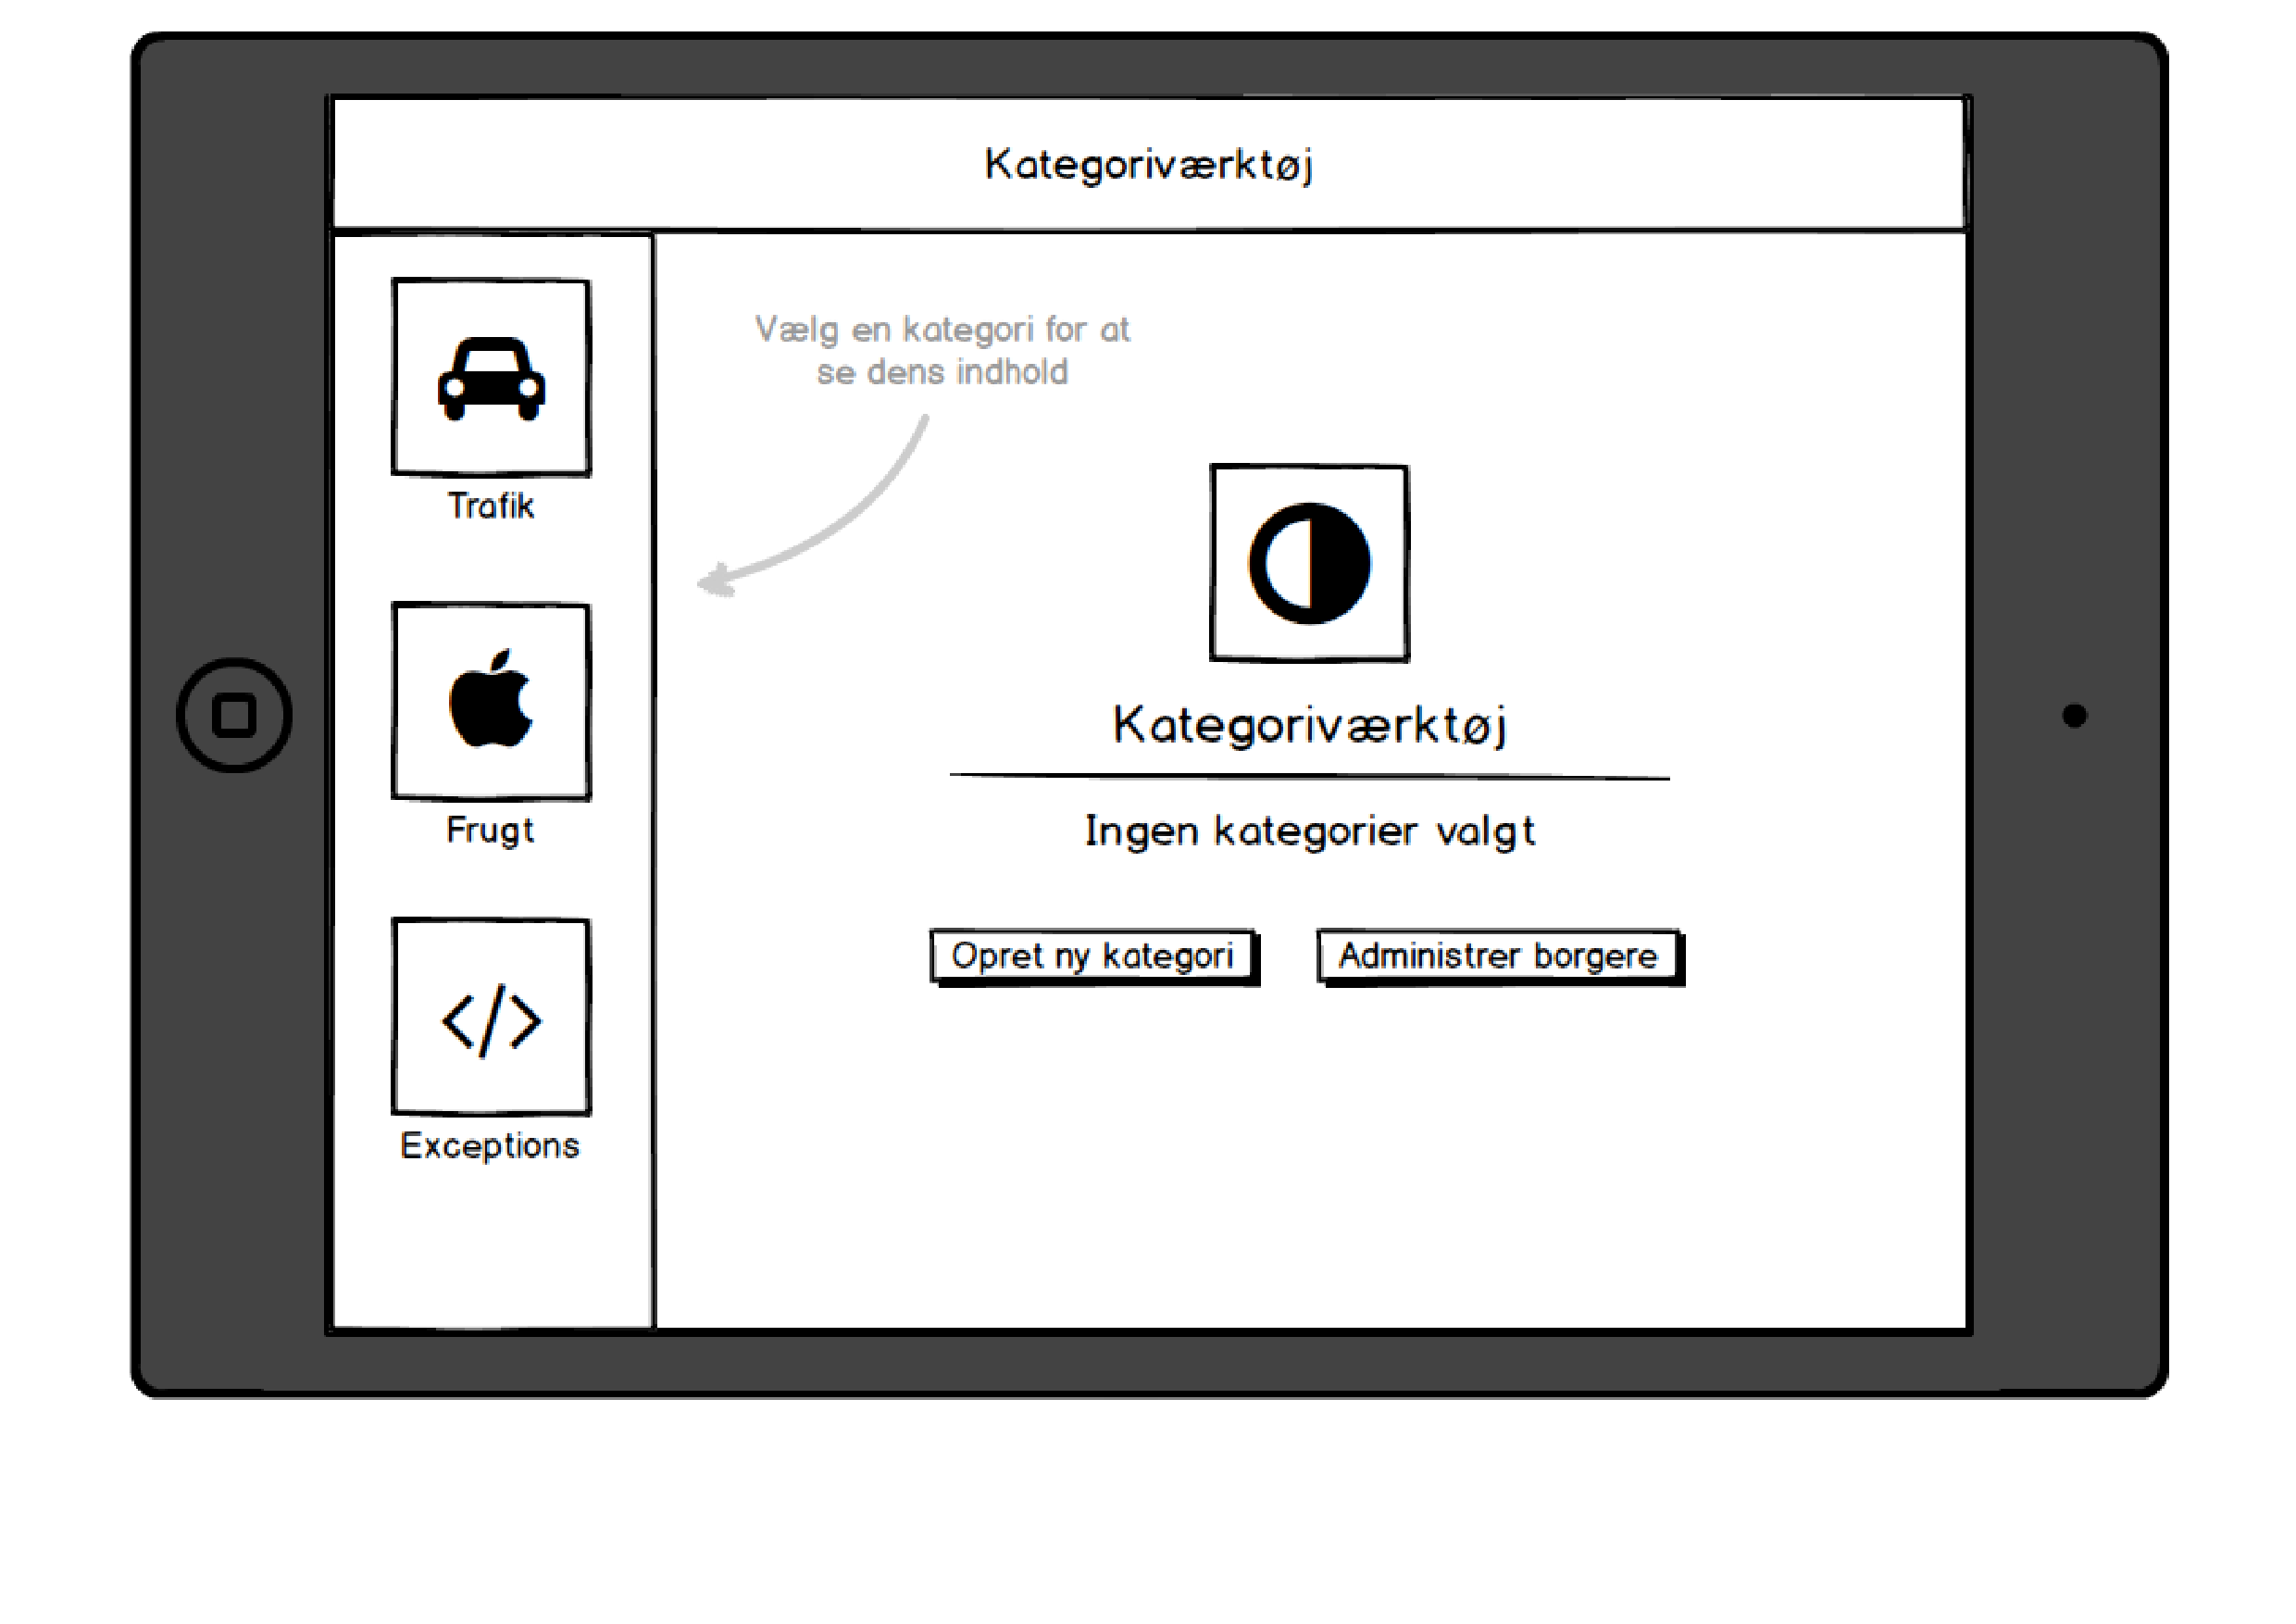
\includegraphics[width=0.75\textwidth]{sprint_two/improved_design/launch_screen}
    \caption{Markup of the launch screen}
    \label{fig:improved_design_launch_screen}
\end{figure}

\subsection{Category Selected Screen}
\label{sec:category_selected_screen}
Whenever the user selected a category (in the menu on the left), a screen very similar to either \figref{fig:improved_design_category_selected_1} or \figref{fig:improved_design_category_selected_2} should be shown (depending on the amount of pictograms in the category).\\

If the category contains no pictograms, a small guide will be shown which will inform the user on how to add pictograms and how to copy the category to users. This will inform users on what the different buttons do. However, if the user is new to the system and needs to work on already existing categories, these buttons could possibly be a bit confusing. \\

\begin{figure}[!htbp]
    \centering
    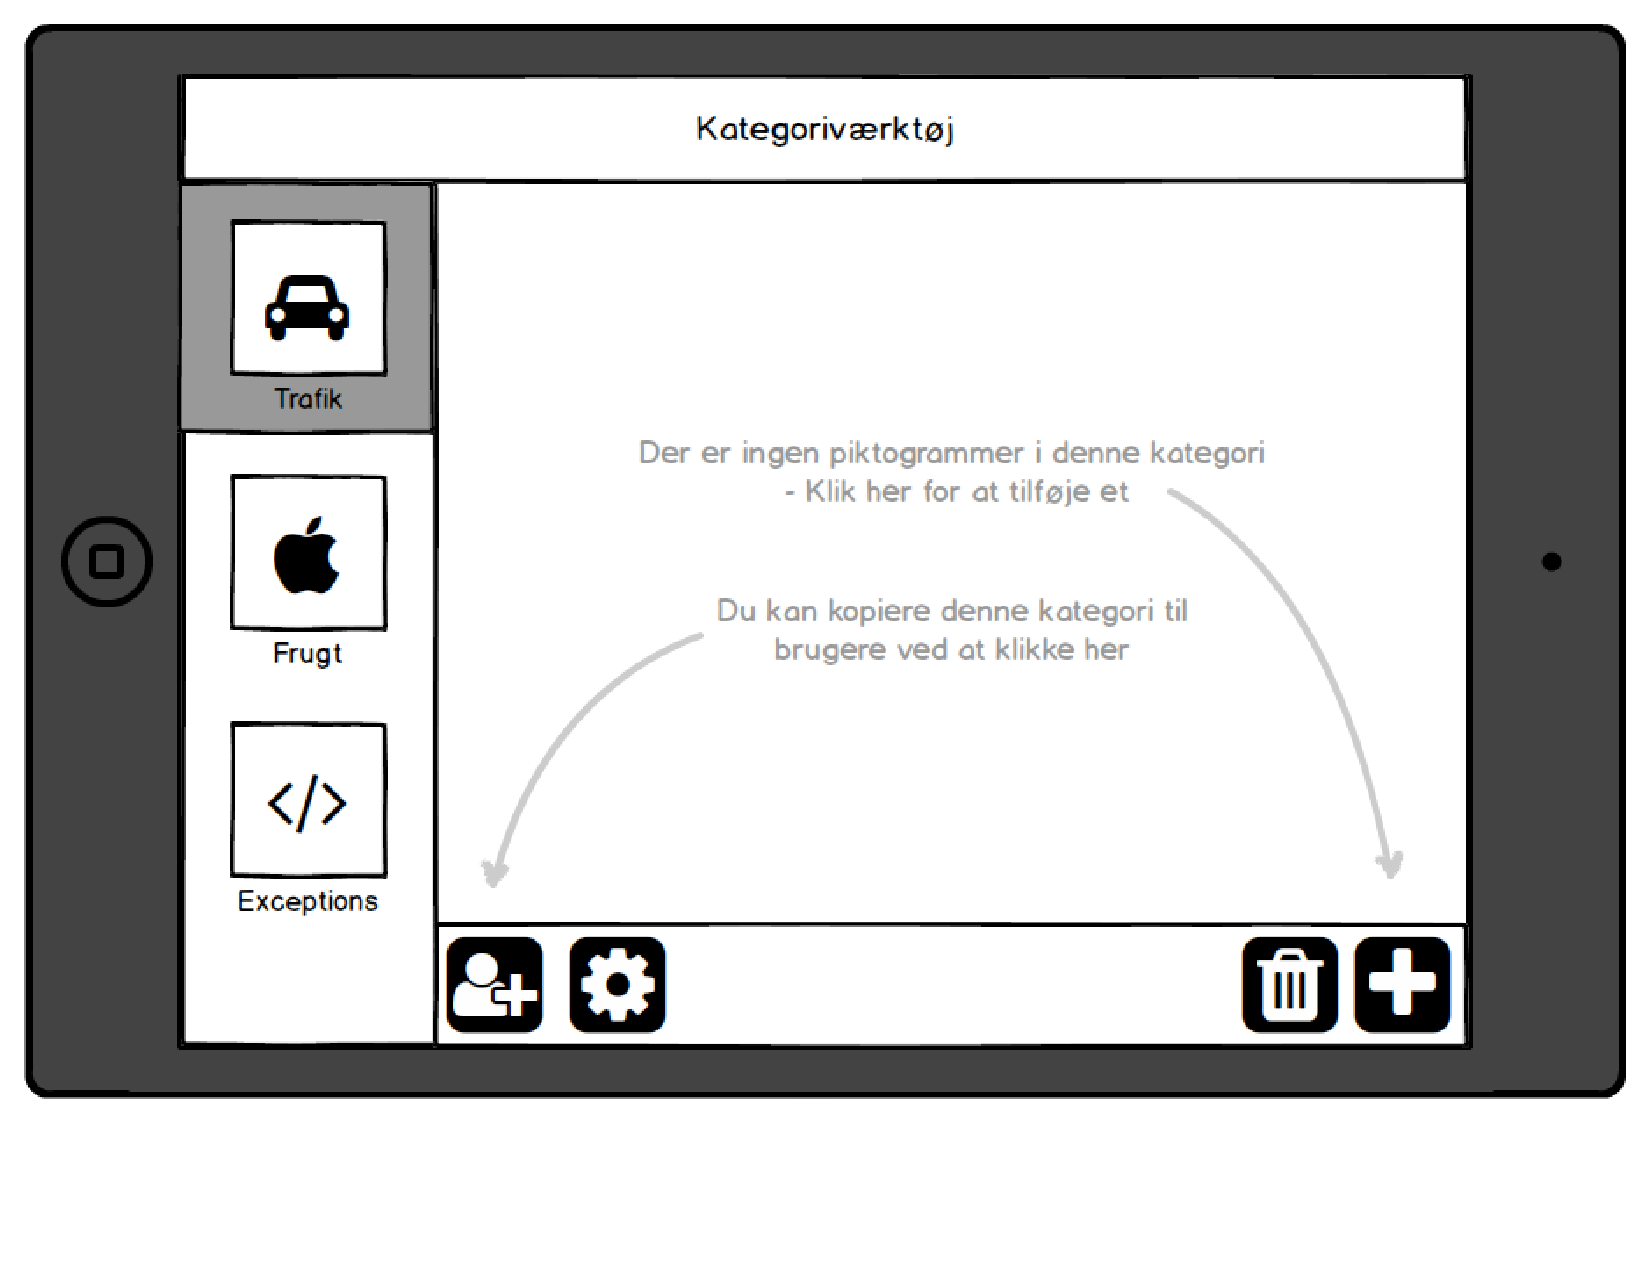
\includegraphics[width=0.75\textwidth]{sprint_two/improved_design/category_selected_1}
    \caption{Markup of the category selected screen without pictograms}
    \label{fig:improved_design_category_selected_1}
\end{figure}

If the category selected contains pictograms, the user will be presented with a screen similar to \figref{fig:improved_design_category_selected_2}. This screen will present the user with a grid of pictogram in the selected category. The user will be able to scroll through the grid if there are more pictograms than available screen estate. 

\begin{figure}[!htbp]
    \centering
    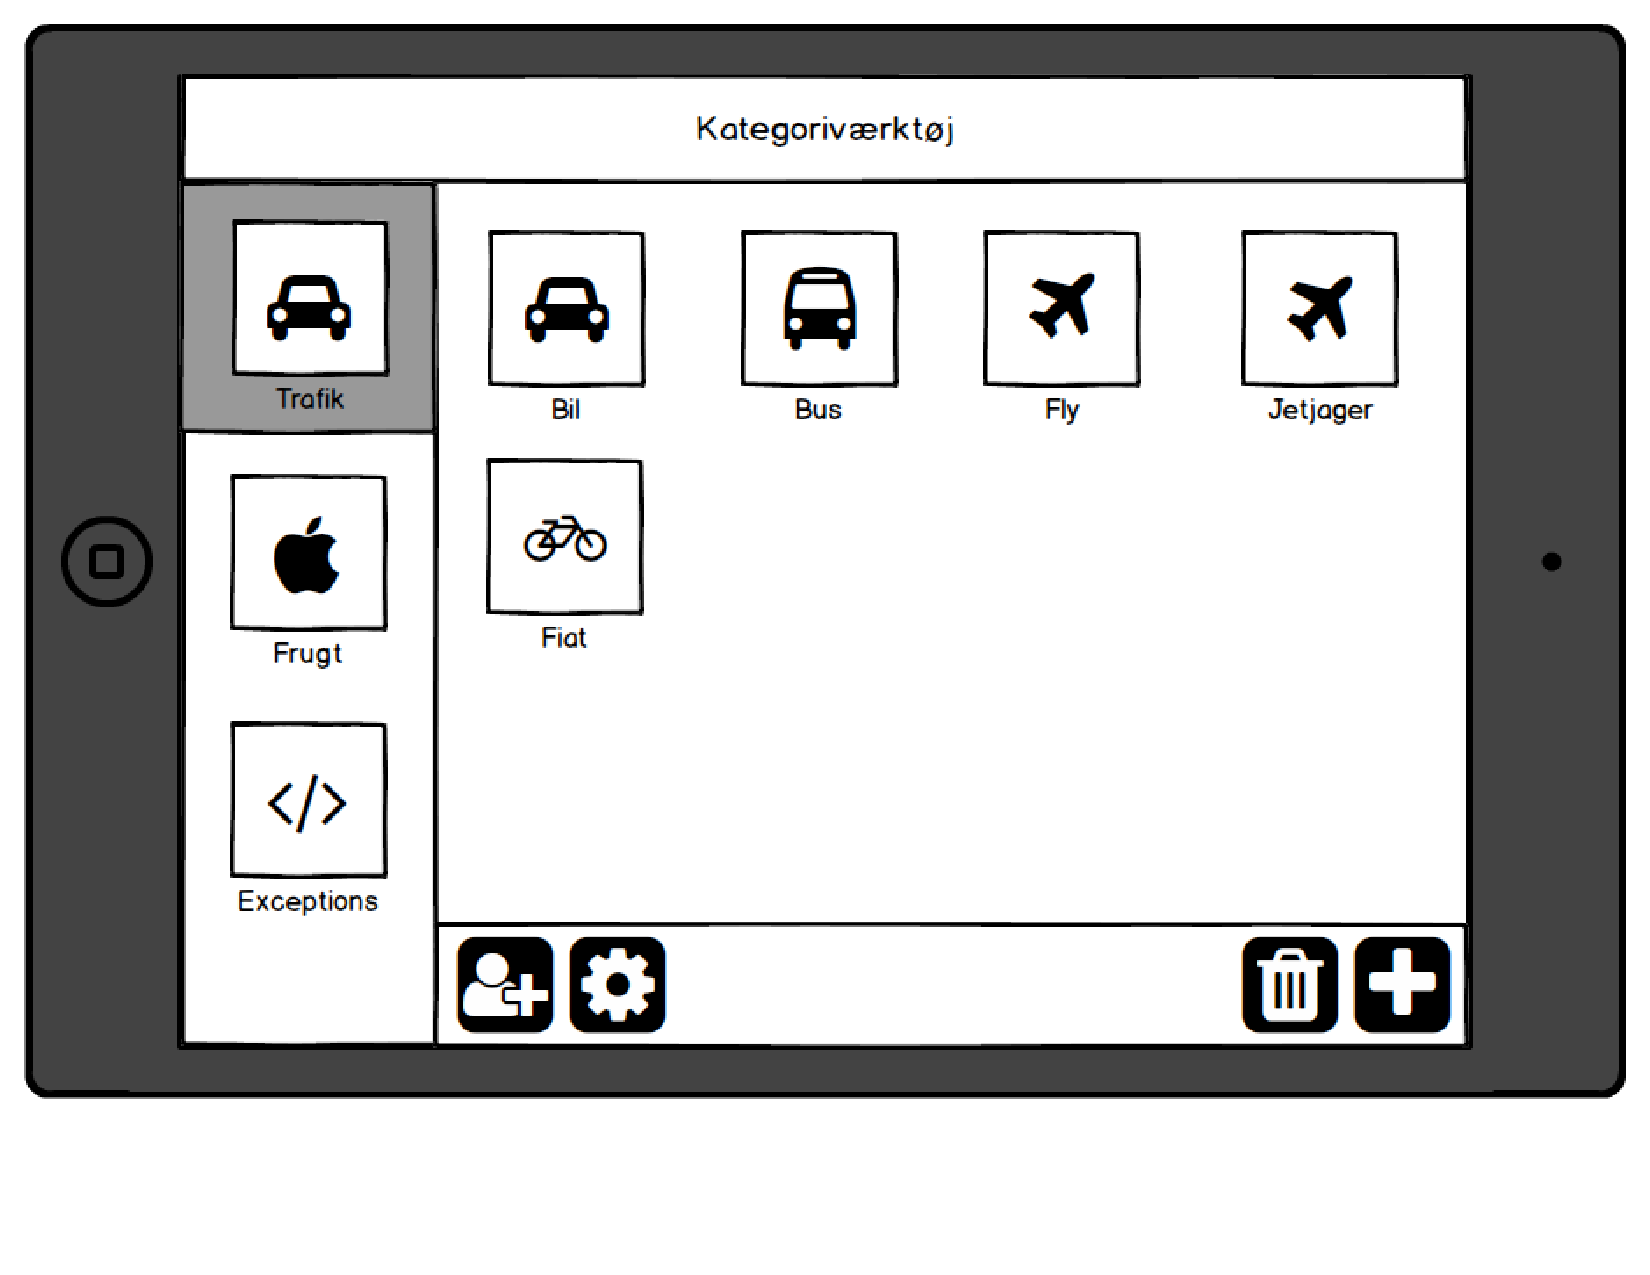
\includegraphics[width=0.75\textwidth]{sprint_two/improved_design/category_selected_2}
    \caption{Markup of the category selected screen with pictograms}
    \label{fig:improved_design_category_selected_2}
\end{figure}

\subsection{Creation and Modification of Categories}
To accommodate the need for creating and removing categories, the following screens have been designed. The category creation screen seen on \figref{fig:improved_design_create_category} will be displayed whenever the \translated{Opret ny kategori}{Create new category} button is pressed. The point of this screen is to guide the user in the creation of a new category. There are two points to consider when creating a category, namely choosing the correct pictogram and picking a eloquent title. To make this very clear to the user, two helping arrows have been added, which reads \translated{Vælg et piktogram}{Skriv en titel} and \translated{Skriv en titel}{Write a title}. These arrows have been added so that the user knows that the pictogram-box is clickable and so that it is clear that you are able to write text in the text-box. 

\begin{figure}[!htbp]
    \centering
    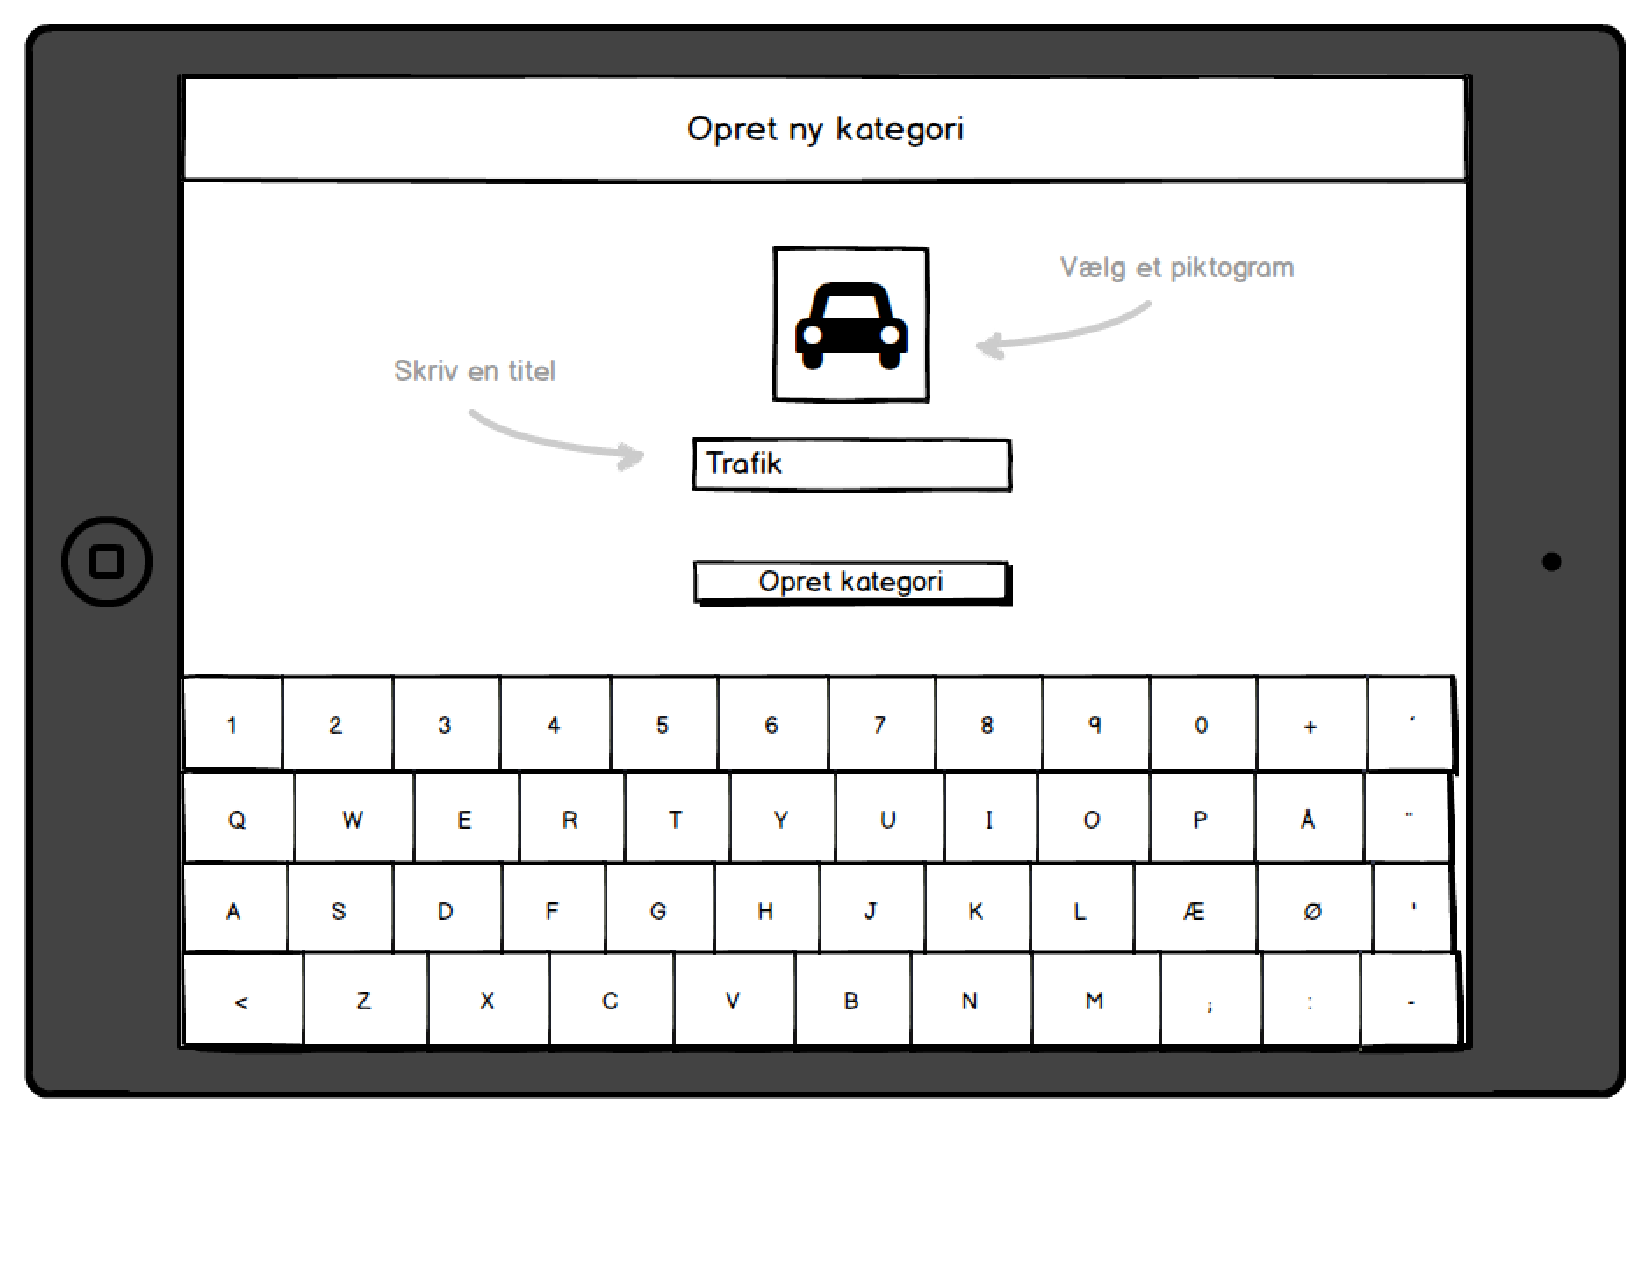
\includegraphics[width=0.75\textwidth]{sprint_two/improved_design/create_category}
    \caption{Markup of the category creation screen}
    \label{fig:improved_design_create_category}
\end{figure}

The user might want to change something regarding a category or deleting the category all together. To do this, the user must first select a category, then press the press the cogwheel on the bottom (see \figref{fig:improved_design_category_selected_2}). This will open the dialog-box shown on \figref{fig:improved_design_category_settings}. Here, the user is presented with two buttons, namely \translated{Slet kategori}{Delete category} and \translated{Gem ændringer}{Save changes}. Furthermore, the user is presented with the helpfull text \translated{Her kan du ændre piktogrammet og titlen for kategorien}{You can change the pictogram and the title for the category}. This dialog does not contain any helpfull arrows, because it was deemed unnessecary at this point since the user should be familiar with the way categories are structured. The only thing that might be problematic with this design is that some users might find it hard to figure out how to get this dialog opened. 

\begin{figure}[!htbp]
    \centering
    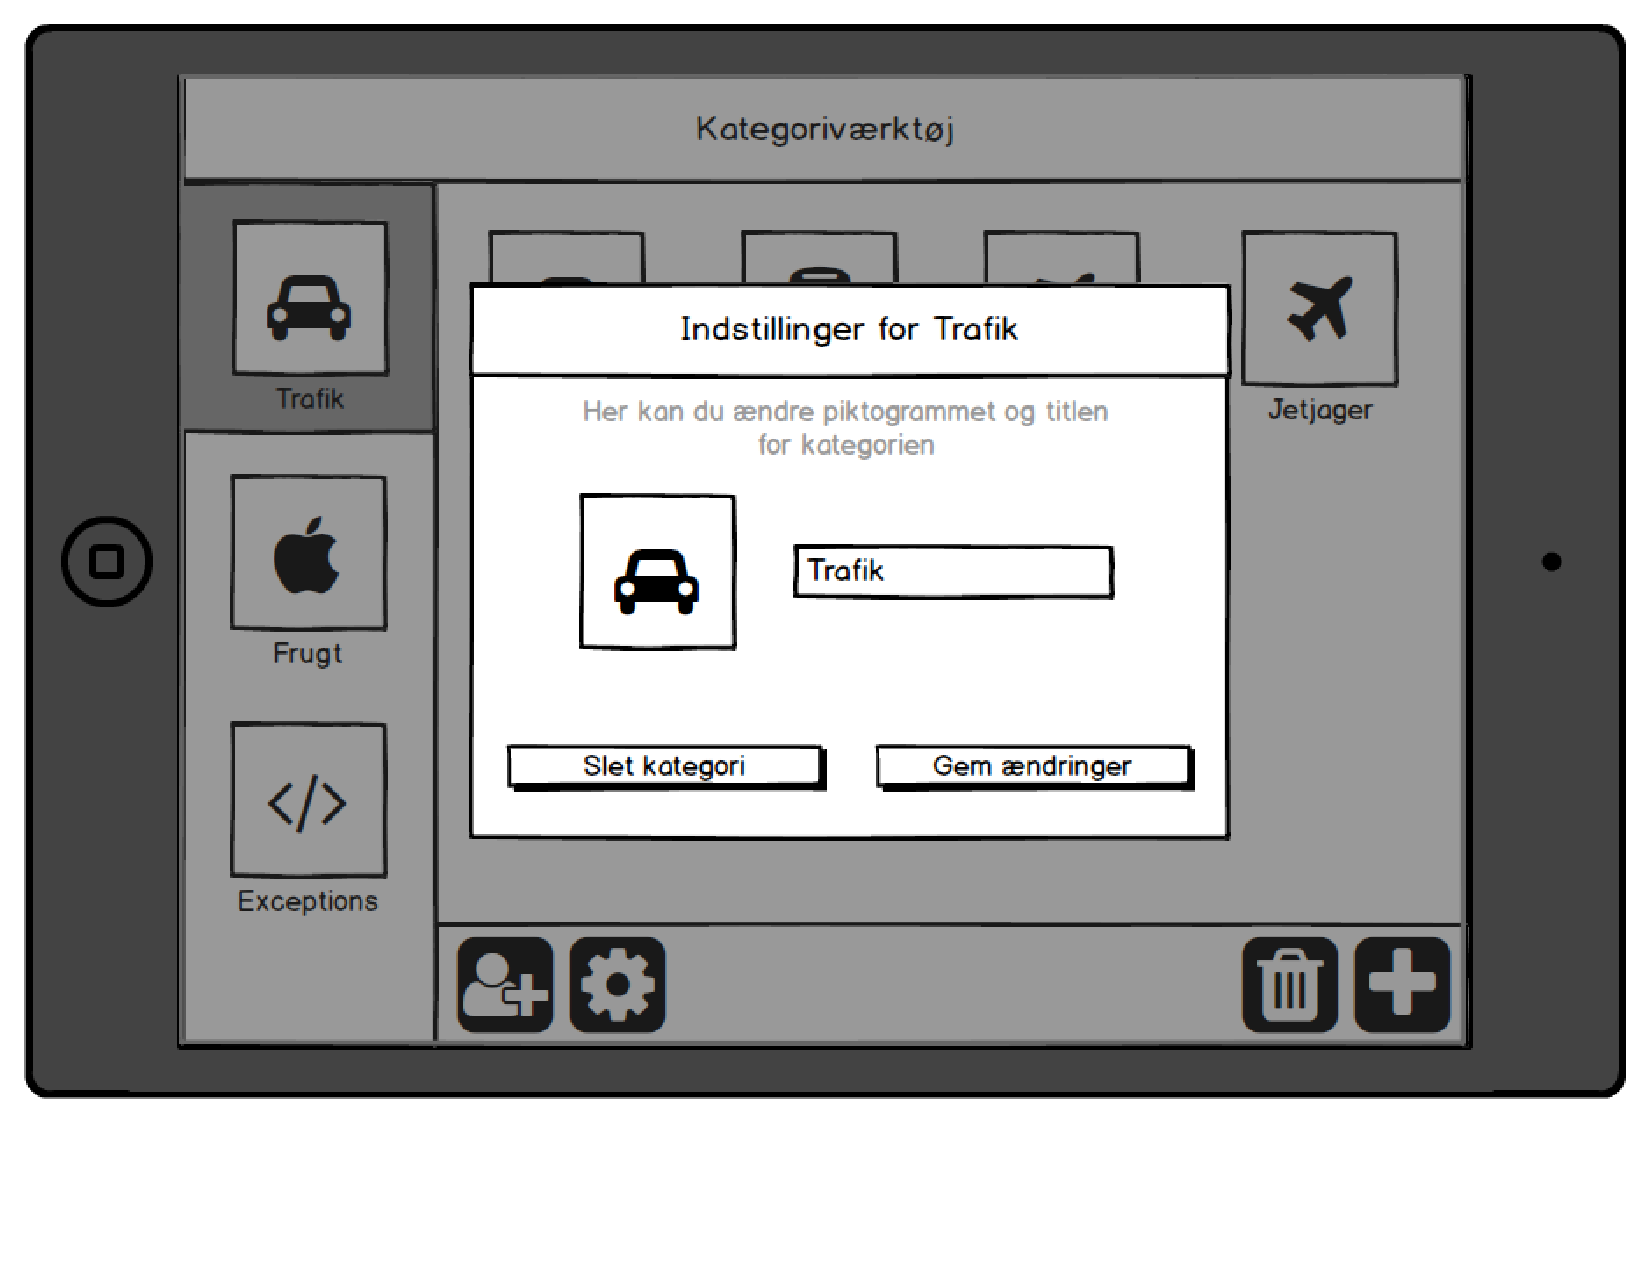
\includegraphics[width=0.75\textwidth]{sprint_two/improved_design/category_settings}
    \caption{Markup of the settings-dialog for a category}
    \label{fig:improved_design_category_settings}
\end{figure}

\FloatBarrier